\section{Trasformata Serie Di Fourier}
    \subsection{Segnale Periodico}
        Si definisce segnale periodico un segnale tale che:
        \[
            x_{(t)} = x_{(t-kT_0)}    
        \]
        \[
            T_0=Periodo\ \ \ f_0\triangleq \frac{1}{T_0} =Frequenza
        \]
    \subsection{Trasformata Serie Di Fourier}
        Ogni segnale periodico di periodo $T_0$ che soddifa le condizioni di Dirichlet e la sua $E_x < \infty (C.S.)$ puó essere scritto come la somma di 
        infinite sinusoidi di frequenze multiple di $f_0 = \frac{1}{T_0}$
        \begin{itemize}
            \item{Equazione di Sintesi - Antitrasformata(ATSF)\label{ATSF}
                \[
                    x_{(t)} = \sum_{k = -\infty}^{\infty} X_{k} e^{j2\pi kf_0t} \hspace{1cm} X_{k}\in \mathbb{C},\ f_0 = \frac{1}{T_0} 
                \]
                Se lo sviluppassimo sarebbe composto da:
                \[
                   x_{(t)} =\ldots  + X_{-1} e^{j2\pi (-1)f_0t} + X_{0} + X_{1} e^{j2\pi (1) f_0t} + \ldots 
                \]
                $X_0$ corrisponde al Valore medio \ref{Valore medio} del segnale, inoltre le componenti $X_k$ prendono il nome di armoniche alla frequenza $f$ corrispondente
            }
            \item{Equazione di Analisi - Trasformata(TSF)\label{TSF}
                \[
                    X_k =\frac{1}{T_0}\int_{-\frac{T_0}{2}}^{\frac{T_0}{2}} x_{(t)} e^{-j2\pi kf_0t} dt
                \]
            } 
        \end{itemize}
        La TSF gode della biunivocitá: $\forall x_{(t)} \exists! X_k$:
        \begin{align}
            x_{(t)} & \overunderset{TSF}{ATSF}{\rightleftharpoons} X_k  \nonumber\\
            Segnale\ Analogico\ Periodico &\overunderset{TSF}{ATSF}{\rightleftharpoons} Sequenza\ Complessa \nonumber
        \end{align}
        \subsubsection{Rappresentazione di $X_k$}
            Essendo $X_k$ un numero complesso puó essere rappresentato in forma polare: 
            \[
                X_k = |X_k|e^{\angle X_k}  
            \]
            Si possono rappresentare il modulo (Ampiezza) e la fase tramite grafici che prendono il nome di spettri:
            \begin{figure}[H]
                \centering
                \subfloat[Spettro di Ampiezza]{
                    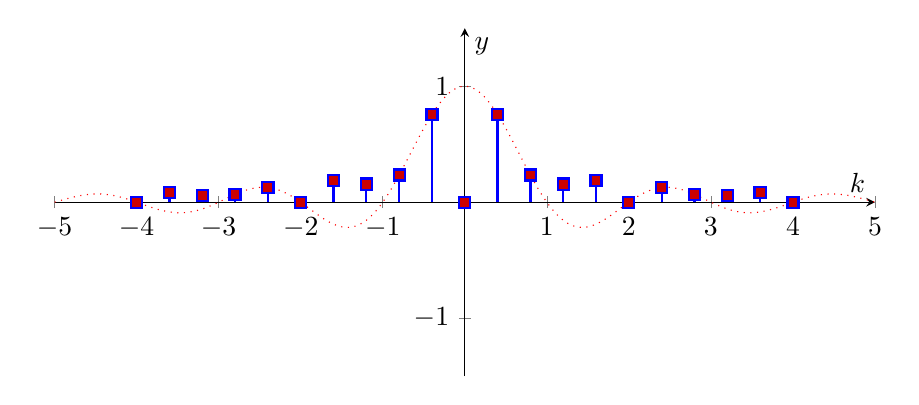
\begin{tikzpicture}
                        \begin{axis}[
                            domain=-5:5,
                            samples=200,
                            axis lines=middle,
                            xlabel=$k$,
                            ylabel=$y$,
                            ymin=-1.5,
                            ymax=1.5,
                            xtick={-5,-4,-3,-2,-1,0,1,2,3,4,5},
                            xticklabels={$-5$,$-4$,$-3$,$-2$,$-1$,$0$,$1$,$2$,$3$,$4$,$5$},
                            ytick={-1, 1},
                            yticklabels={$-1$, $1$},
                            width=12cm,
                            height=6cm
                        ]
                        \addplot [red,dotted, samples = 300] {sin(deg(x*pi))/(x*pi)};
                        \addplot+ [blue, thick, ycomb, samples at={-4,-3.6,-3.2,-2.8,-2.4,-2,-1.6,-1.2,-0.8,-0.4,0,0.4,0.8,1.2,1.6,2,2.4,2.8,3.2,3.6,4}] {abs(sin(deg(x*pi))/(x*pi))};
                        \end{axis}
                    \end{tikzpicture}
                }
                \hfill
                \subfloat[Spettro di Fase]{
                    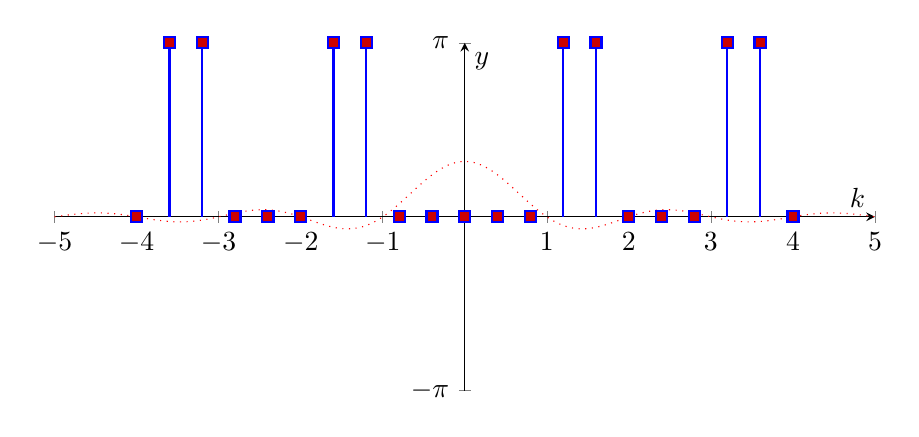
\begin{tikzpicture}
                        \begin{axis}[
                            domain=-5:5,
                            samples=200,
                            axis lines=middle,
                            xlabel=$k$,
                            ylabel=$y$,
                            ymin=-pi,
                            ymax=pi,
                            xtick={-5,-4,-3,-2,-1,0,1,2,3,4,5},
                            xticklabels={$-5$,$-4$,$-3$,$-2$,$-1$,$0$,$1$,$2$,$3$,$4$,$5$},
                            ytick={-pi, pi},
                            yticklabels={$-\pi$, $\pi$},
                            width=12cm,
                            height=6cm
                        ]
                        \addplot [red,dotted, samples = 300] {sin(deg(x*pi))/(x*pi)};
                        \addplot+ [blue, thick, ycomb, samples at={-4,-3.6,-3.2,-2.8,-2.4,-2,-1.6,-1.2,-0.8,-0.4,0,0.4,0.8,1.2,1.6,2,2.4,2.8,3.2,3.6,4}] {rad(atan2(0,sin(deg(x*pi))/(x*pi)))};
                        \end{axis}
                    \end{tikzpicture}
                }
                \caption{Spettro di un treno di rect}
            \end{figure}
            lo spettro di Ampiezza gode della \textbf{simmetria pari} rispetto alle ascisse quindi é \textbf{sempre positivo}, mentre lo spettro di fase della \textbf{simmetria dispari}.
        \subsection{Propietá della TSF}
            \subsection{Linearitá}
            \subsection{Simmetria Hermitiana}
        
        \subsection{Calcolo dei coefficenti $X_k$ per segnali noti}
            \subsubsection{$A\cos(2\pi f_0 t)$}
                $x_{(t)}=A\cos(2\pi f_0 t), \hspace{0.3cm} A>0$
                \begin{align}
                    ATSF[x_{(t)}] & = ATSF[A\cos(2\pi f_0 t)] \nonumber \\
                        & = ATSF[\frac{A}{2} (e^{j2\pi kf_0t} + e^{-j2\pi kf_0t})] \nonumber 
                \end{align}
                Utilizzando la composizione dei coefficenti $X_k$:
                \begin{align}
                    x_{(t)} & =\ldots  + X_{-1} e^{j2\pi (-1)f_0t} + X_{0} + X_{1} e^{-j2\pi (1) f_0t} + \ldots \nonumber\\
                    Abbiamo:& \nonumber 
                \end{align}
                        \[X_{-1} = \frac{A}{2}\hspace{.3cm} X_{0} = 0\hspace{.3cm} X_{1} = \frac{A}{2}\] 
                Possiamo tracciare lo spettro del segnale:
                \begin{figure}[H]
                    \centering
                    \subfloat[Spettro di Ampiezza]{
                    \begin{tikzpicture}
                        \begin{axis}[
                            domain=-4:4,
                            samples=200,
                            axis lines=middle,
                            xlabel=$t$,
                            ylabel=$y$,
                            ymin=-1.5,
                            ymax=1.5,
                            xtick={-5,-4,-3,-2,-1,0,1,2,3,4,5},
                            xticklabels={$-5$,$-4$,$-3$,$-2$,$-1$,$0$,$1$,$2$,$3$,$4$,$5$},
                            ytick={1},
                            yticklabels={$\frac{A}{2}$},
                            width=6.5cm,
                            height=5cm
                            ]
                            \addplot [const plot,black,dotted] coordinates{(-4,1)(4,1)};
                            \addplot+ [blue, thick, ycomb, samples at = {-1,1}] {1};
                            \end{axis}
                        \end{tikzpicture}
                    }
                    \hfill
                    \subfloat[Spettro di Fase]{
                        \begin{tikzpicture}
                            \begin{axis}[
                                domain=-4:4,
                                samples=200,
                                axis lines=middle,
                                xlabel=$t$,
                                ylabel=$y$,
                                ymin=-pi,
                                ymax=pi,
                                xtick={-5,-4,-3,-2,-1,0,1,2,3,4,5},
                                xticklabels={$-5$,$-4$,$-3$,$-2$,$-1$,$0$,$1$,$2$,$3$,$4$,$5$},
                                ytick={-pi, pi},
                                yticklabels={$-\pi$, $\pi$},
                                width=6.5cm,
                                height=5cm
                            ]
                            \addplot+ [blue, thick, ycomb, samples at = {-4,-3,-2,-1,0,1,2,3,4}] {0};
                            \end{axis}
                        \end{tikzpicture}
                    }
                    \caption{Spettro TSF del coseno $A>0$}
                \end{figure}
            \subsubsection{$A\sin(2\pi f_0 t)$}
                $x_{(t)}=A\sin(2\pi f_0 t), \hspace{0.3cm} A>0$
                \begin{align}
                    ATSF[x_{(t)}] & = ATSF[A\sin(2\pi f_0 t)] \nonumber \\
                        & = ATSF[\frac{A}{2} (e^{j2\pi kf_0t} - e^{-j2\pi kf_0t})] \nonumber 
                \end{align}
                Utilizzando la composizione dei coefficenti $X_k$:
                \begin{align}
                    x_{(t)} & =\ldots  + X_{-1} e^{j2\pi (-1)f_0t} - X_{0} + X_{1} e^{-j2\pi (1) f_0t} + \ldots \nonumber\\
                    Abbiamo:& \nonumber 
                \end{align}
                        \[X_{-1} = -\frac{A}{2j}\hspace{.3cm} X_{0} = 0\hspace{.3cm} X_{1} = \frac{A}{2j}\] 
                \[
                    |X_k|= 
                    \begin{cases}
                            |\frac{A}{2j}| = \frac{A}{2} \hspace{0.5cm} & k= 1\\
                            |-\frac{A}{2j}| = \frac{A}{2} \hspace{0.5cm} & k= -1\\
                            0 \hspace{0.5cm} & altrove  \\
                    \end{cases}
                    \hspace{0.5cm}
                    \angle X_k= 
                    \begin{cases}
                        \angle \frac{A}{2j} = -\frac{\pi}{2} \hspace{0.5cm} & k= 1\\
                        \angle |-\frac{A}{2j}| = \frac{\pi}{2} \hspace{0.5cm} & k= -1\\
                        0 \hspace{0.5cm} & altrove  \\
                    \end{cases}
                    \]
                Possiamo tracciare lo spettro del segnale:
                \begin{figure}[H]
                    \centering
                    \subfloat[Spettro di Ampiezza]{
                        \begin{tikzpicture}
                            \begin{axis}[
                                domain=-4:4,
                                samples=200,
                                axis lines=middle,
                                xlabel=$t$,
                                ylabel=$y$,
                                ymin=-1.5,
                                ymax=1.5,
                                xtick={-5,-4,-3,-2,-1,0,1,2,3,4,5},
                                xticklabels={$-5$,$-4$,$-3$,$-2$,$-1$,$0$,$1$,$2$,$3$,$4$,$5$},
                                ytick={1},
                                yticklabels={$\frac{A}{2}$},
                                width=6.5cm,
                                height=5cm
                                ]
                                \addplot [const plot,black,dotted] coordinates{(-4,1)(4,1)};
                                \addplot+ [blue, thick, ycomb, samples at = {-1,1}] {1};
                                \end{axis}
                            \end{tikzpicture}
                        }
                    \hfill
                    \subfloat[Spettro di Fase]{
                            \begin{tikzpicture}
                                \begin{axis}[
                                    domain=-4:4,
                                    samples=200,
                                    axis lines=middle,
                                    xlabel=$t$,
                                    ylabel=$y$,
                                    ymin=-pi,
                                    ymax=pi,
                                    xtick={-5,-4,-3,-2,-1,0,1,2,3,4,5},
                                    xticklabels={$-5$,$-4$,$-3$,$-2$,$-1$,$0$,$1$,$2$,$3$,$4$,$5$},
                                    ytick={-pi,-1/2*pi,1/2*pi, pi},
                                    yticklabels={$-\pi$,$-\frac{\pi}{2}$,$\frac{\pi}{2}$ $\pi$},
                                    yticklabel style = {xshift=3pt}, 
                                    width=6.5cm,
                                    height=5cm
                                ]
                                \addplot+ [blue, thick,const plot] coordinates{(-1,1/2*pi)(-1,0)};
                                \addplot+ [blue, thick,const plot] coordinates{(1,-1/2*pi)(1,0)};

                                \addplot [black, dotted,const plot] coordinates{(-3,-1/2*pi)(3,-1/2*pi)};
                                \addplot [black, dotted,const plot] coordinates{(-3,1/2*pi)(3,1/2*pi)};
                                \end{axis}
                            \end{tikzpicture}
                        }
                    \caption{Spettro TSF del seno $A>0$}
                \end{figure}
            \subsubsection{Treno di rect}
                $x_R=A\hspace{0.1cm}rect\left(\frac{t}{T}\right)\rightarrow$ Segnale periodico $\rightarrow x_{(t)} = \sum_{-\infty}^{\infty} x_R (t-nT_0)$\\
                $T_0 = periodo$, $T = durata \rightarrow T < T_0$, se cosi non fosse avremmo una costante
                \begin{figure}[H]
                    \centering
                    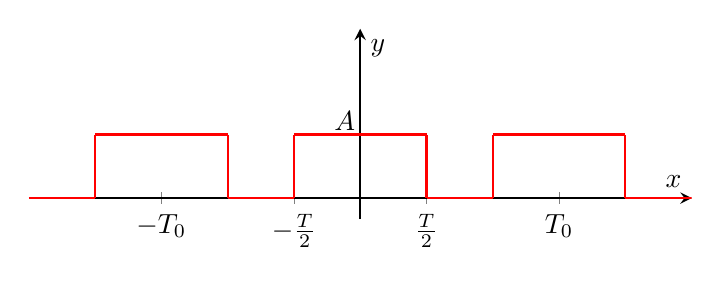
\begin{tikzpicture}
                        \begin{axis}[
                            xlabel=$x$,
                            ylabel=$y$,
                            xmin=-5,
                            xmax=5,
                            ymin=-0.5,
                            ymax=4,
                            ytick = {1.5},
                            xtick={-3,-1, 0, 1,3},
                            xticklabels={$-T_0$,$-\frac{T}{2}$, $0$, $\frac{T}{2}$,$T_0$},
                            yticklabels = {$A$},
                            yticklabel style = {yshift=5pt,xshift=4pt}, 
                            axis lines=middle,
                            thick,
                            domain=-5:5,
                            samples=100,
                            width=10cm,
                            height=4cm
                        ]
                        \addplot [const plot,red, thick] coordinates{(-1,1.5)(1,1.5)};
                        \addplot [const plot,red, thick] coordinates{(-1,0)(-1,1.5)};
                        \addplot [const plot,red, thick] coordinates{(1,0)(1,1.5)};
                        
                        \addplot [const plot,red, thick] coordinates{(-2,1.5)(-4,1.5)};
                        \addplot [const plot,red, thick] coordinates{(-2,0)(-2,1.5)};
                        \addplot [const plot,red, thick] coordinates{(-4,0)(-4,1.5)};
                        
                        \addplot [const plot,red, thick] coordinates{(2,1.5)(4,1.5)};
                        \addplot [const plot,red, thick] coordinates{(2,0)(2,1.5)};
                        \addplot [const plot,red, thick] coordinates{(4,0)(4,1.5)};
                        
                        \addplot [const plot,red, thick] coordinates{(2,0)(1,0)};
                        \addplot [const plot,red, thick] coordinates{(-2,0)(-1,0)};
                        \addplot [const plot,red, thick] coordinates{(-4,0)(-5,0)};
                        \addplot [const plot,red, thick] coordinates{(4,0)(5,0)};
                    
                        \end{axis}
                    \end{tikzpicture}
                    \caption{Treno di $A\hspace{0.1cm}rect\left(\frac{t}{T}\right)$}
                    \label{fig:treno di rect}
                \end{figure}                
                $\rightarrow$ Si nota come cambiare il periodi delle funzioni possiamo renderle da aperiodiche a periodiche e viceversa
                \begin{align}
                    ATSF[x_{(t)}] & = ATSF[\sum_{-\infty}^{\infty} x_R (t-nT_0)] \nonumber \\
                        & = \frac{1}{T_0} \int_{-\frac{T_0}{2}}^{\frac{T_0}{2}} x_{(t)} e^{-j2\pi kf_0t} dt = \frac{1}{T_0} \int_{-\frac{T}{2}}^{\frac{T}{2}} x_{(t)} e^{-j2\pi kf_0t} dt \nonumber \\
                        & = \frac{A}{T_0} \int_{-\frac{T}{2}}^{\frac{T}{2}} e^{-j2\pi kf_0t} dt = \eval{\frac{A}{T_0} \frac{1}{j2\pi kf_0} e^{-j2\pi kf_0t}}_{-\frac{T}{2}}^{\frac{T}{2}} \nonumber \\
                        & = \frac{A}{T_0} \frac{e^{-j\pi kf_0T} - e^{j\pi kf_0T}}{j2\pi kf_0} = \frac{A}{T_0} \frac{e^{j\pi kf_0T}-e^{-j\pi kf_0T}}{-j2\pi kf_0} \nonumber \\
                        & = \frac{A\color{purple}{T}}{T_0} \frac{e^{j\pi kf_0T}-e^{-j\pi kf_0T}}{-j2\pi kf_0\color{purple}{T}} = Af_0T sinc(kf_0T) \nonumber 
                \end{align}
                Tracciamo lo spettro per $f_0T<1$:
                \begin{figure}[H]
                    \centering
                    \subfloat[Spettro di Ampiezza]{
                        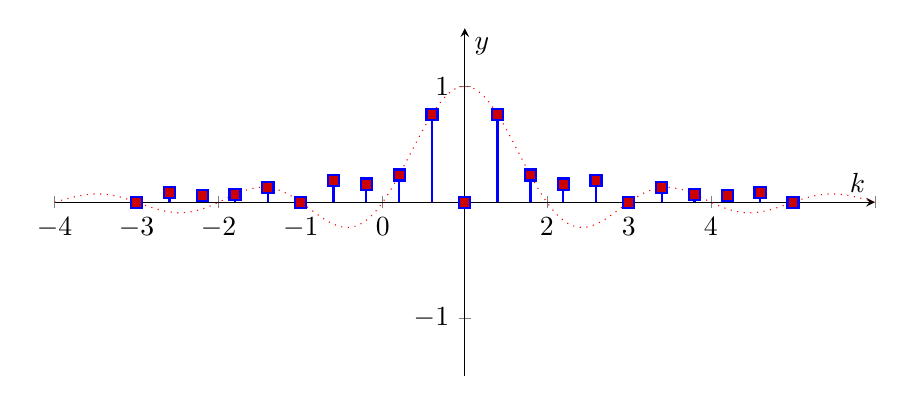
\begin{tikzpicture}
                            \begin{axis}[
                                domain=-5:5,
                                samples=200,
                                axis lines=middle,
                                xlabel=$k$,
                                ylabel=$y$,
                                ymin=-1.5,
                                ymax=1.5,
                                xtick={-5,-4,-3,-2,-1,0,1,2,3,4,5},
                                xticklabels={$-4$,$-3$,$-2$,$-1$,$0$,$1$,$2$,$3$,$4$},
                                ytick={-1, 1},
                                yticklabels={$-1$, $1$},
                                width=12cm,
                                height=6cm
                            ]
                            \addplot [red,dotted, samples = 300] {sin(deg(x*pi))/(x*pi)};
                            \addplot+ [blue, thick, ycomb, samples at={-4,-3.6,-3.2,-2.8,-2.4,-2,-1.6,-1.2,-0.8,-0.4,0,0.4,0.8,1.2,1.6,2,2.4,2.8,3.2,3.6,4}] {abs(sin(deg(x*pi))/(x*pi))};
                            \end{axis}
                        \end{tikzpicture}
                    }
                    \hfill
                    \subfloat[Spettro di Fase]{
                        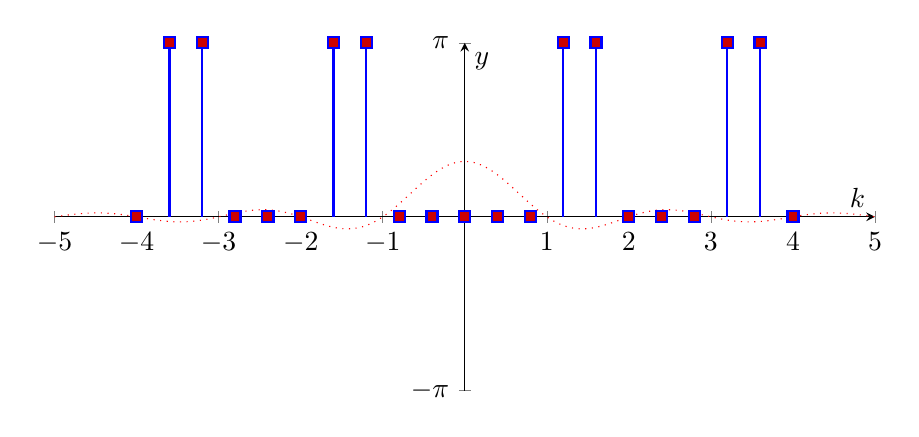
\begin{tikzpicture}
                            \begin{axis}[
                                domain=-5:5,
                                samples=200,
                                axis lines=middle,
                                xlabel=$k$,
                                ylabel=$y$,
                                ymin=-pi,
                                ymax=pi,
                                xtick={-5,-4,-3,-2,-1,0,1,2,3,4,5},
                                xticklabels={$-5$,$-4$,$-3$,$-2$,$-1$,$0$,$1$,$2$,$3$,$4$,$5$},
                                ytick={-pi, pi},
                                yticklabels={$-\pi$, $\pi$},
                                width=12cm,
                                height=6cm
                            ]
                            \addplot [red,dotted, samples = 300] {sin(deg(x*pi))/(x*pi)};
                            \addplot+ [blue, thick, ycomb, samples at={-4,-3.6,-3.2,-2.8,-2.4,-2,-1.6,-1.2,-0.8,-0.4,0,0.4,0.8,1.2,1.6,2,2.4,2.8,3.2,3.6,4}] {rad(atan2(0,sin(deg(x*pi))/(x*pi)))};
                            \end{axis}
                        \end{tikzpicture}
                    }
                    \caption{Spettro TSF del treno di rect con $f_0T<1$}
                \end{figure}
                Si possono anche unire i due spettri per ottenere: 
                \begin{figure}[H]
                    \centering
                    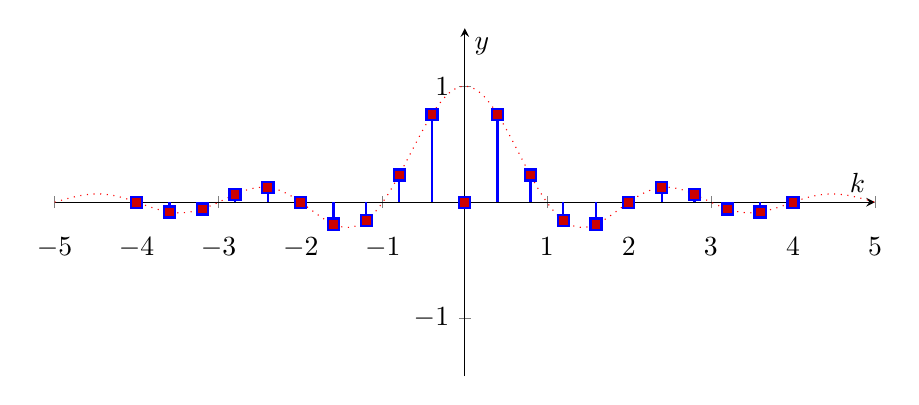
\begin{tikzpicture}
                        \begin{axis}[
                            domain=-5:5,
                            samples=200,
                            axis lines=middle,
                            xlabel=$k$,
                            ylabel=$y$,
                            ymin=-1.5,
                            ymax=1.5,
                            xtick={-5,-4,-3,-2,-1,0,1,2,3,4,5},
                            xticklabels={$-5$,$-4$,$-3$,$-2$,$-1$,$0$,$1$,$2$,$3$,$4$,$5$},
                            ytick={-1, 1},
                            yticklabels={$-1$, $1$},
                            xticklabel style = {yshift=-7pt}, 
                            width=12cm,
                            height=6cm
                        ]
                        \addplot [red,dotted, samples = 300] {sin(deg(x*pi))/(x*pi)};
                        \addplot+ [blue, thick, ycomb, samples at={-4,-3.6,-3.2,-2.8,-2.4,-2,-1.6,-1.2,-0.8,-0.4,0,0.4,0.8,1.2,1.6,2,2.4,2.8,3.2,3.6,4}] {sin(deg(x*pi))/(x*pi)};
                        \end{axis}
                    \end{tikzpicture}
                    \caption{Spettro treno di $A\hspace{0.1cm}rect\left(\frac{t}{T}\right)$}
                    \label{fig:Spettro treno di rect}
                \end{figure}  
            Ora appizza matlab e fa esempi di un segnale e uno di riostruzione dello stesso(script di matlab presenti nel teams):
            \begin{itemize}
                \item Se un segnale varia molto rapidamente nel tempo ha componenti frequenziali piú alte $\rightarrow$ copre piú spettro(espansione spettrale) $T_0 \uparrow$
                \item Se un segnale varia molto lentamente copre le basse fraquenze $ T_0 \downarrow$
            \end{itemize}
            Se non ho abbastanza passi K non posso campionare le alte frequenze e quindi non faccio ne un analisi completa del segnale né riesco a ricostruire perfettametne il segnale  
            Inoltre in $0$ dello spettro ho il Valor medio \ref{Valore medio} del segnale